\documentclass{article}
\usepackage[utf8]{inputenc}
\usepackage[margin=4cm]{geometry}
\usepackage{graphicx}

\title{Assignment B -- On Paper}
\author{Eirik Isene}
\date{\today}

\begin{document}

\maketitle

\section{From the book}
\subsection{Excercise 3.3, Page 56}
If you wanted to search for {\tt s*ng} in a permuterm wildcard index, what key(s) would one do the lookup on? \\ \\
Before rotating the term {\tt s*ng} wer mark the end to make it {\tt s*ng\$}, then we rotate it so that we can treat it as a trailing wildcard query, the resulting key to use in a search is then: {\tt ng\$s*}
\subsection{Excercise 3.8, Page 62}
Compute the edit distance between {\tt paris} and {\tt alice}. Write down the $5 \times 5$ array of distances between all prefixes as computed by the algorithm in Figure 3.5 \\ \\
\begin{center}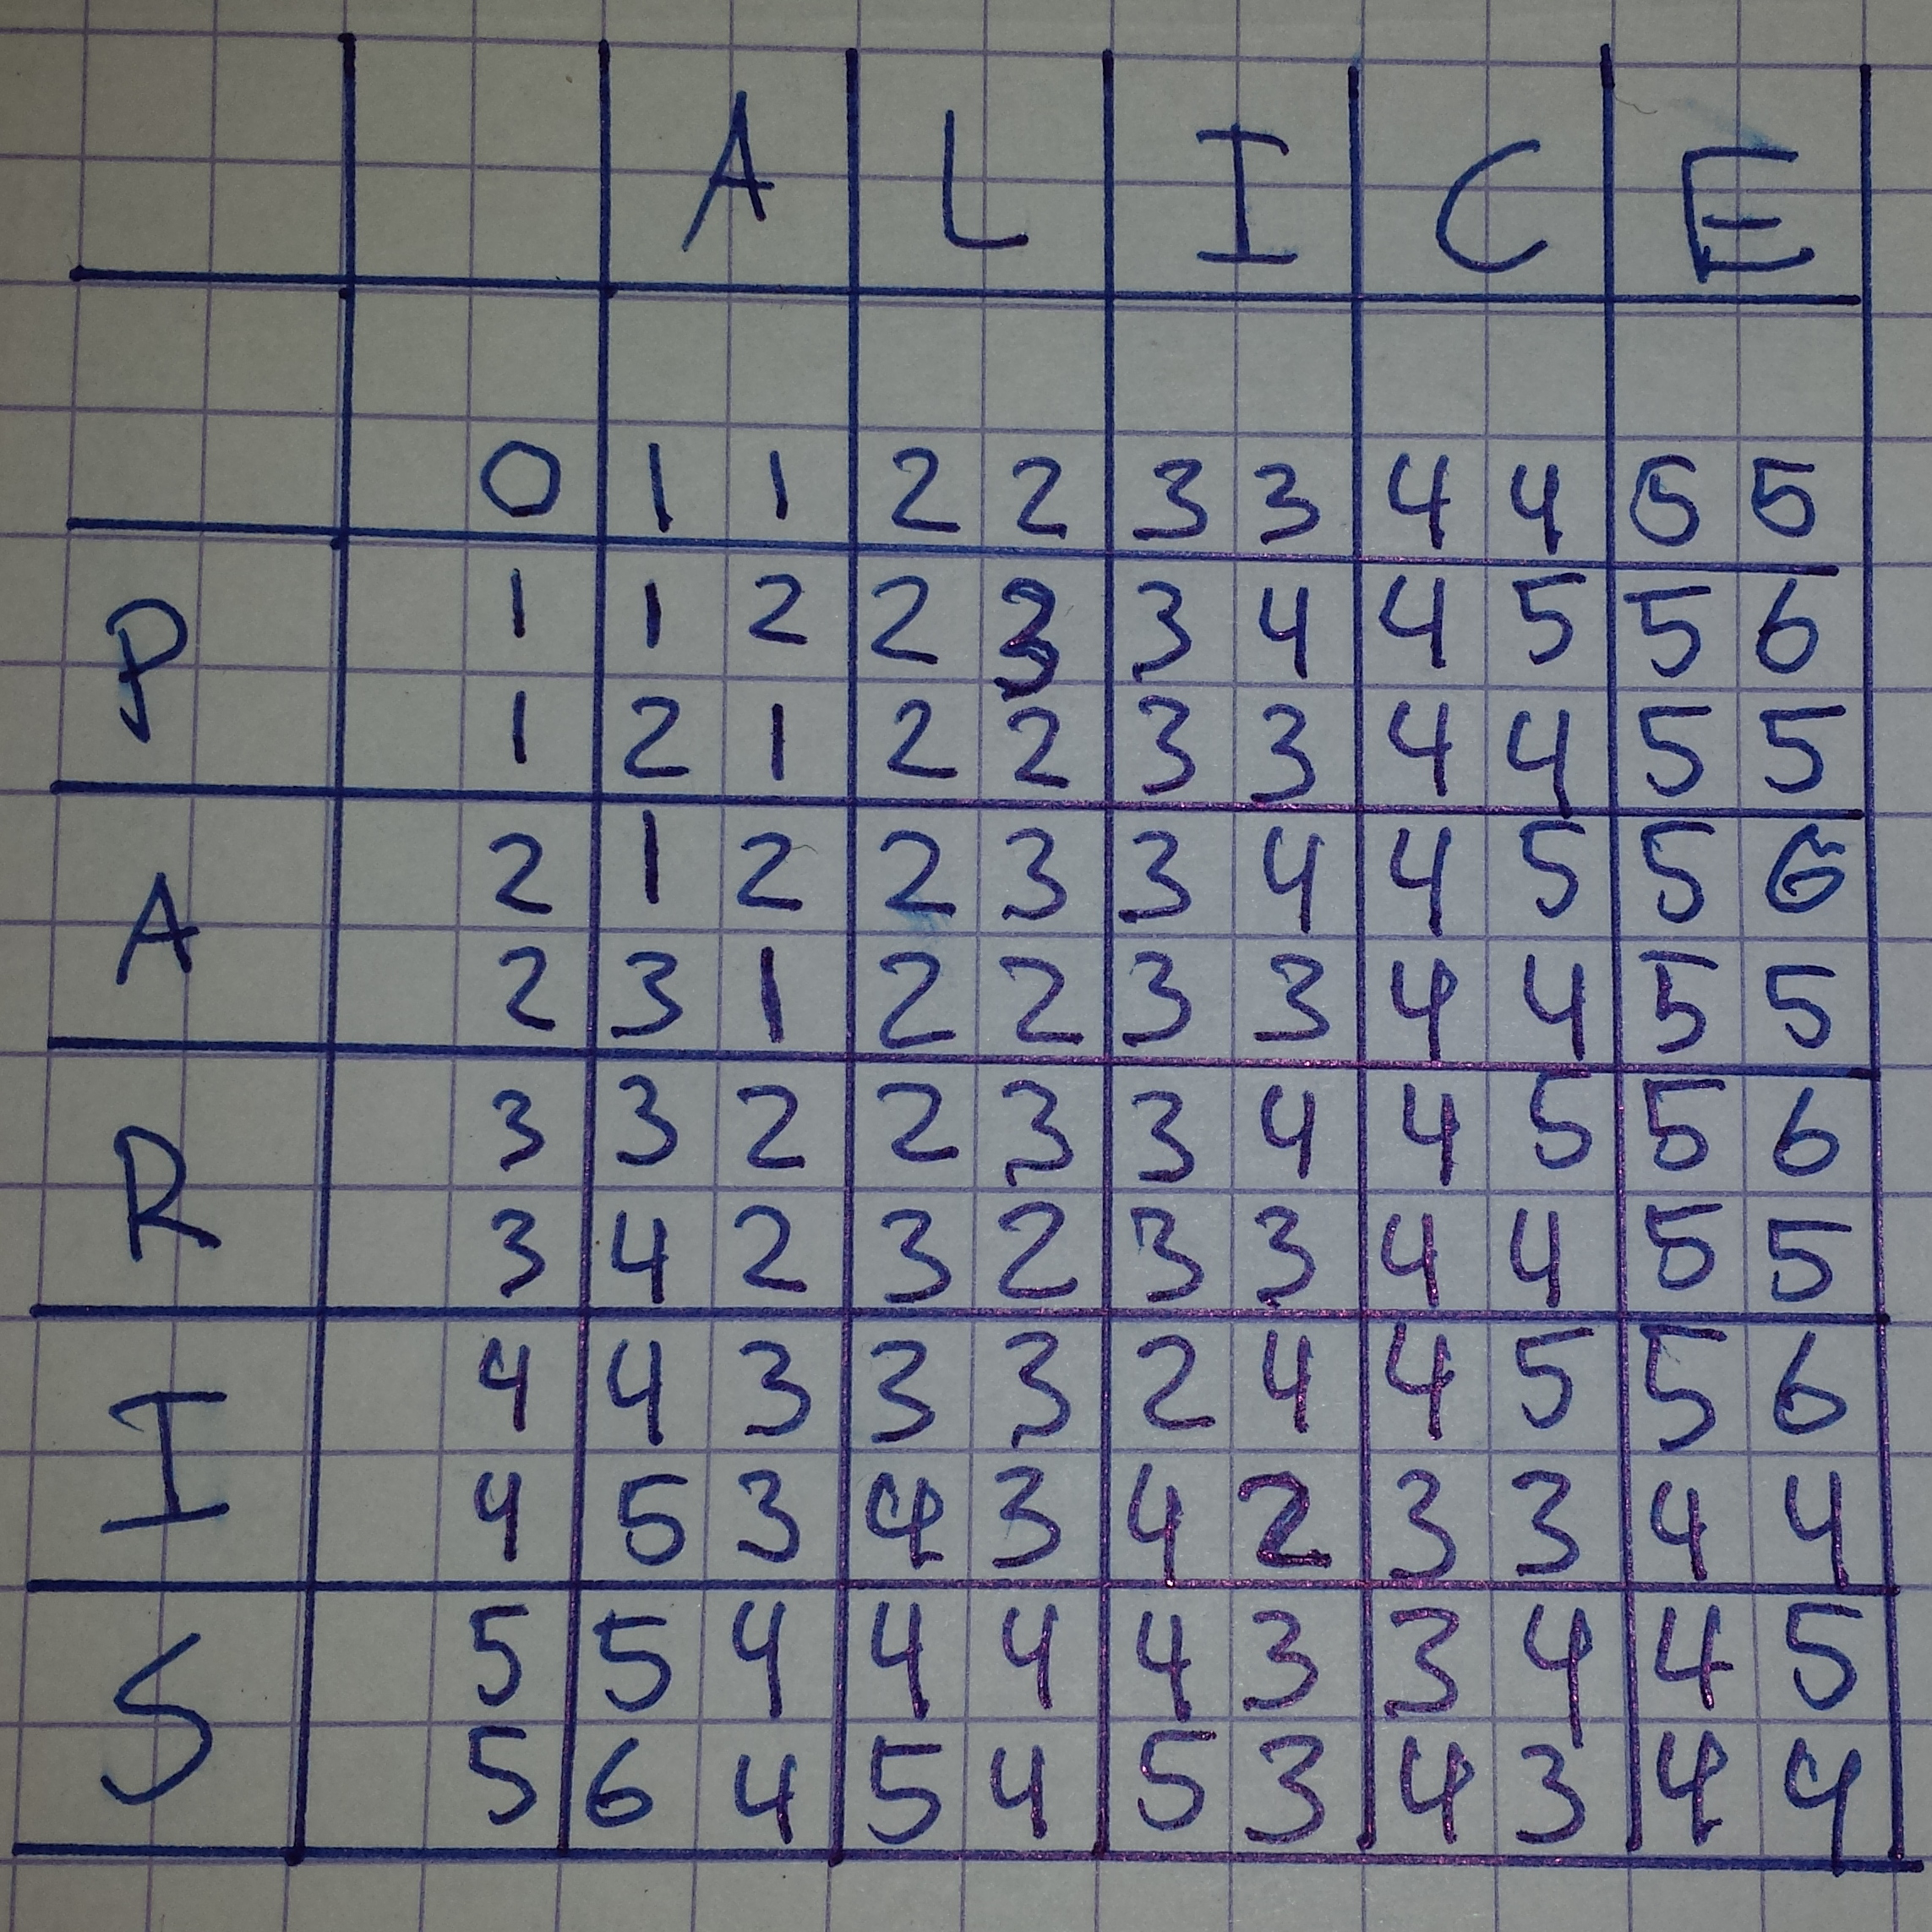
\includegraphics[width=8cm]{editDistance.jpg}\end{center}
\section{String matching algorithms}

\subsection{Kurts large dicitionary}
Kurt has a large dictionary with millions of elements. As part of a document processing system, he wants to develop a module which can efficiently detect whether a word in a document is also present in the dictionary.
\subsubsection{What data structure should Kurt use to represent his dictionary?}
I would recommend Kurt to use a Trie to represent the dictionary. This makes finding words in the dictionary a simple and efficient operation. It will also save space since a lot of the words in the dictionary wil have common prefixes that share nodes in the trie structure. It would also be wise to tightly pack the trie, this way not only the prefixes are shared, but also the suffixes. For a large dictionary this will save a lot of space!
\subsubsection{What algorithm should be used to search the data structure?}
To search the data structure a Trie walk algorithm should be used.

\subsection{Kurts spellchecking}
Kurt also has a big dictionary containing the surface forms of the most common words in Norwegian. As part of a spellchecking application, Kurt wants to be able to query the dictionary with a word $w$ and get back the set of all words which have an edit distanec of at most $k$ from $w$. More formally, the resulting set is thus defined as $$\{w': editdistance(w',w) <= k \}$$ You can assume that the maximum distance $k$ is small.
\subsubsection{How should Kurt represent his dictionary and perform the search?}
Seeing as words following the same path in a Trie have the same prefix, a Trie should still be used for this. When finding words that have edit distance within the limitations, one can calculate columns in the edit table until the edit distance exceeds the limitation, and cut away all branches from there and out since the edit distance won't decrease further down. This way we can easilly present a section of a trie where the edit distance is within limitations from one word to another. 

\end{document}
